\subsection{Implementering af boundry klasser}
Til at implemtere broundry klasserne i systemet benyttes XML-filer, der håndteres i deres respektive controllere. I disse filer er det muligt at definere, hvilke type elemtenter, der skal indgå i layoutet. Dertil kan typen af layout defineres alt efter, hvordan layoutet skal opstilles. Layouts brugt i dette system er af type linear og relativ layout.  

Elementer opstilles i layouts med type, størrelse samt orientering. Forekommer det, at elementerne skal benyttes i javekoden, defineres disse ligeledes med et id. Et eksempel af layoutkode fra log ind ses af \autoref{fig:logindlay}.

\begin{figure} [H]
\centering
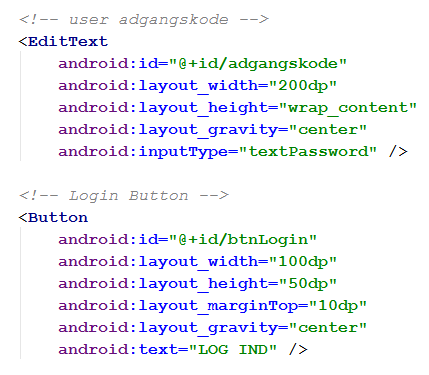
\includegraphics[width=0.8\textwidth]{figures/logindlay}
\caption{Udklip af kode fra log ind layout. Udklippet viser et edittext, hvori brugeren angiver adgangskode samt en button for log ind.}
\label{fig:logindlay}
\end{figure}

Af dette udklip ses koden for tekstfeltet, hvori brugeren angiver adgangskode samt koden for layoutet af log ind-knappen. Feltet for adgangskoden er her af typen EditText, der tillader, at brugeren kan angive tekst. Dette felt har ligeledes et id, der muliggører at referere til feltet og hente den angivet adgangskode til validering af log ind. Knappen er opstillet af typen button, og har ligeledes et id, hvortil en listener er opstillet i javakoden. 
